\subsection{\secState{D}Storm}\label{s:testStorm}
    \paragraph{Scenario:} Small UAS is flying in open space in uncontrolled airspace ($\le$ 500 feet AGL (Above Ground Level)). A \emph{Weather Service} notices UAS about \emph{Dangerous Weather zone} (virtual constraint s. \ref{s:virtualConstraints}) which is moving in UAS direction. The \emph{UAS} is  executing mission given by (tab. \ref{tab:missionSetupStormScenario}).
    
    \begin{table}[H]
        \centering
        \begin{tabular}{c|c||c}
            \multicolumn{2}{c||}{Position} & \multirow{2}{*}{$\mathscr{WP}_1$} \\\cline{1-2}
            $[x,y,z]$           & $[\theta,\varpi,\psi]$           & \\\hline\hline
            $[0,0,0]^T $        & $[0^\circ,0^\circ,90^\circ]^T$    & $[0,60,0]^T$        \\ 
        \end{tabular}
        \caption{Mission setup for \emph{Storm} scenario.}
        \label{tab:missionSetupStormScenario}
    \end{table}
    
    \paragraph{Constraints:} The \emph{storm} is modeled as a \emph{virtual constraint} with parameters given in (tab. \ref{tab:obstacleSetStorm}). A constraint is modeled as a \emph{convex polygon} for \emph{horizontal boundary} and altitude for the \emph{vertical boundary}.
    
    The \emph{Storm} is moving through an \emph{operational region} with linear velocity $0.5 ms^{-1}$. The \emph{storm`s center} was first detected at \emph{decision frame} $0$ at position $[0,50,0]^T$.
    
    \begin{table}[H]
        \centering
        \begin{tabular}{c|c|c|c|c|c|c}
            \multicolumn{3}{c|}{Constraint} & \multicolumn{3}{c|}{Body Margin} & \multirow{2}{*}{Safety Margin}\\\cline{1-6}
            i. position & velocity & type & min. & max. & avg. &   \\\hline\hline
            $[0,50,0]^T$ & $[0,-0.5,0]$ & polygon & $9$ & $10$ & $9.5$  & $5$ \\
         \end{tabular}
        \caption{\emph{Constraint set} for \emph{Storm} scenario.}
        \label{tab:obstacleSetStorm}
    \end{table}
    
    \paragraph{Assumption:} Every \emph{avoidable moving constraint} is usually slower than an \emph{Approaching UAS}, or its radius is smaller than the turning radius of an \emph{Approaching UAS}.
    
    \begin{note}
    \emph{Manned aviation} receives a permit to operate in  \emph{controlled airspace} only if it has capability outmaneuver every known threat in requested airspace. 
    
    The \emph{Constrained space portion} is usually very large, therefore in the majority of cases the assumption $uasSpeed >> constraintSpeed$  holds.
    \end{note}
 
    \paragraph{Main Goal:} Show dynamic moving constraint avoidance capability in \emph{uncontrolled airspace}.
    
    \paragraph{Acceptance criteria:}
    \begin{enumerate}
        \item \emph{Hard constraint avoidance} - the \emph{UAS} must not cross the body margin:  $distance($ $stormCenter,$ $UAS)$ $\ge$  $bodyMargin$.
        
        \item \emph{Soft constraint avoidance} - the \emph{UAS} cannot cross the safety margin to get into proximity of \emph{Storms surrounding area}: \emph{distance(stormCenter, UAS)} $\ge$ \emph{safetyMargin}. 
    \end{enumerate}
    
    \paragraph{Testing setup:} The \emph{standard test setup} defined in (tab. \ref{tab:testMovementOrientations}, \ref{tab:testUASBasicParameters}, \ref{tab:testNavigationGridBasic}, \ref{tab:testAvoidanceGridBasic}, \ref{tab:testUASColoring}) is used with following parameter override:
    \begin{enumerate}
        \item \emph{Avoidance grid - type} - \emph{ACAS-like} with \emph{horizontal enabled maneuvers}.
    \end{enumerate}
    
    \paragraph{Simulation run:} \emph{Notable moments} from a \emph{simulation run} (fig. \ref{fig:testCaseStormAvoidance}) are the following:
    \begin{enumerate}
    
        \item \emph{Detection} (fig. \ref{fig:stromSituationDetection}) - the \emph{Storm} (magenta polygon) is detected prior to the engagement (retrieved from associated weather service). The \emph{UAS} (blue) stays in \emph{Navigation mode}. \emph{Trajectories} in \emph{Navigation grid} are constrained by rule \emph{Enforce safety margin} (tab. \ref{tab:ruleEnforceSafetyMargin}). The \emph{Planned trajectory} (red) changes to avoid \emph{Storm}.
        
        \item \emph{Avoidance start} (fig. \ref{fig:stormAvoidanceStart}) - when UAS reaches optimal avoidance distance, the \emph{navigation reach set} is constrained, forcing UAS to perform an evasive maneuver.
        
        \item \emph{Avoidance end} (fig. \ref{fig:stormAvoidanceEnd}) - navigation space is no longer constrained when the \emph{minimal safe distance/heading} is achieved.
        
        \item \emph{Waypoint reached} (fig. \ref{fig:stormWaypointReach}) - standard waypoint navigation procedure was used in this case.
        
    \end{enumerate}
        
    \begin{figure}[H]
        \centering
        \begin{subfigure}{0.48\textwidth}
        	\centering
            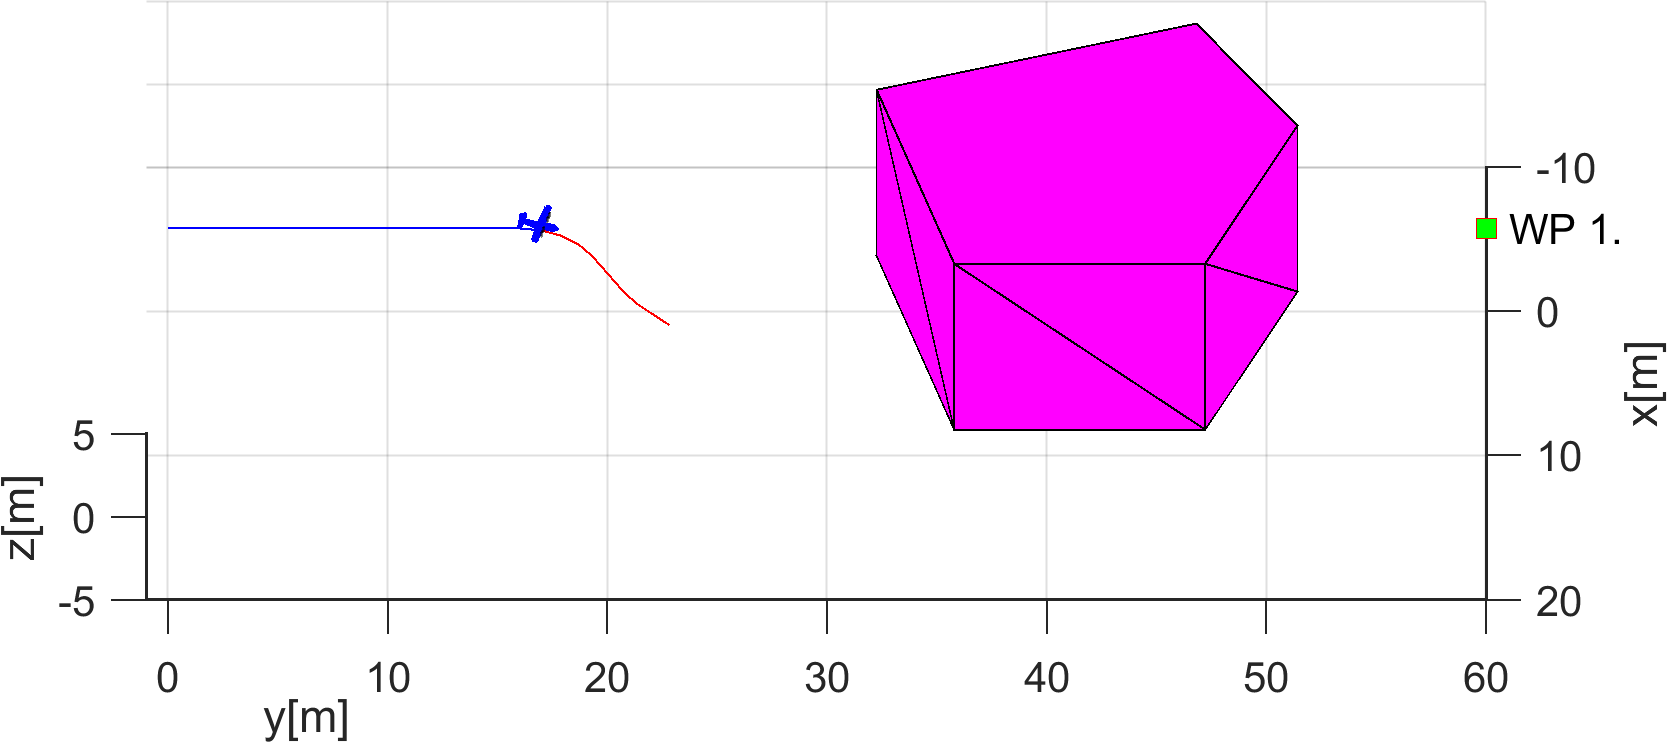
\includegraphics[width=0.9\linewidth]{\FIGDIR/NS019ConstraintsPolynomialStorm00017}
            \caption{Situation detection.}
            \label{fig:stromSituationDetection}
        \end{subfigure}
        \begin{subfigure}{0.48\textwidth}
        	\centering
            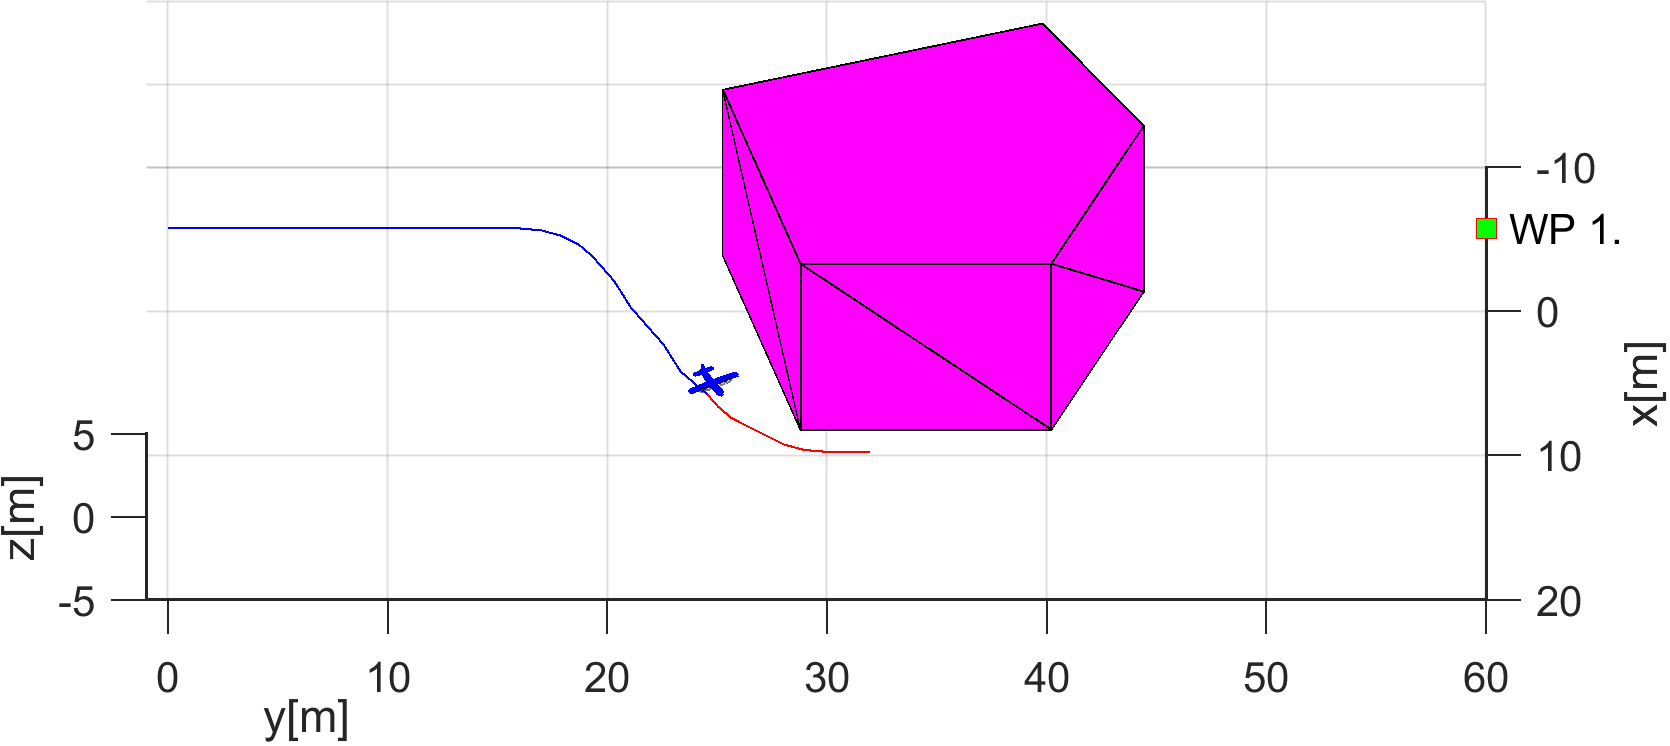
\includegraphics[width=0.9\linewidth]{\FIGDIR/NS020ConstraintsPolynomialStorm00031} 
            \caption{Storm avoidance start.}
            \label{fig:stormAvoidanceStart}
        \end{subfigure}
        \\
        \begin{subfigure}{0.48\textwidth}
        	\centering
            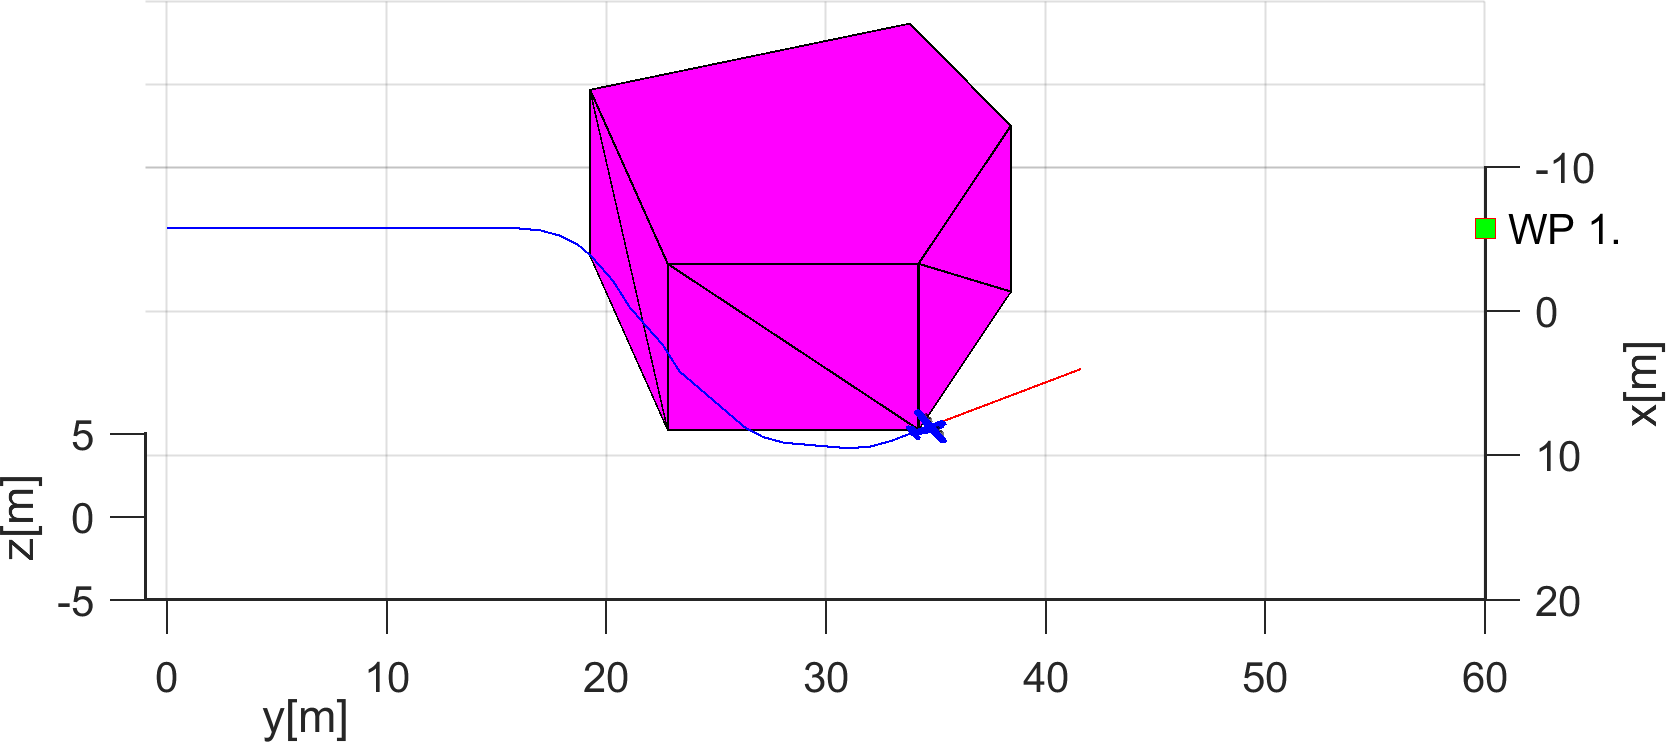
\includegraphics[width=0.9\linewidth]{\FIGDIR/NS021ConstraintsPolynomialStorm00043} 
            \caption{Storm avoidance end.}
            \label{fig:stormAvoidanceEnd}
        \end{subfigure}
        \begin{subfigure}{0.48\textwidth}
        	\centering
            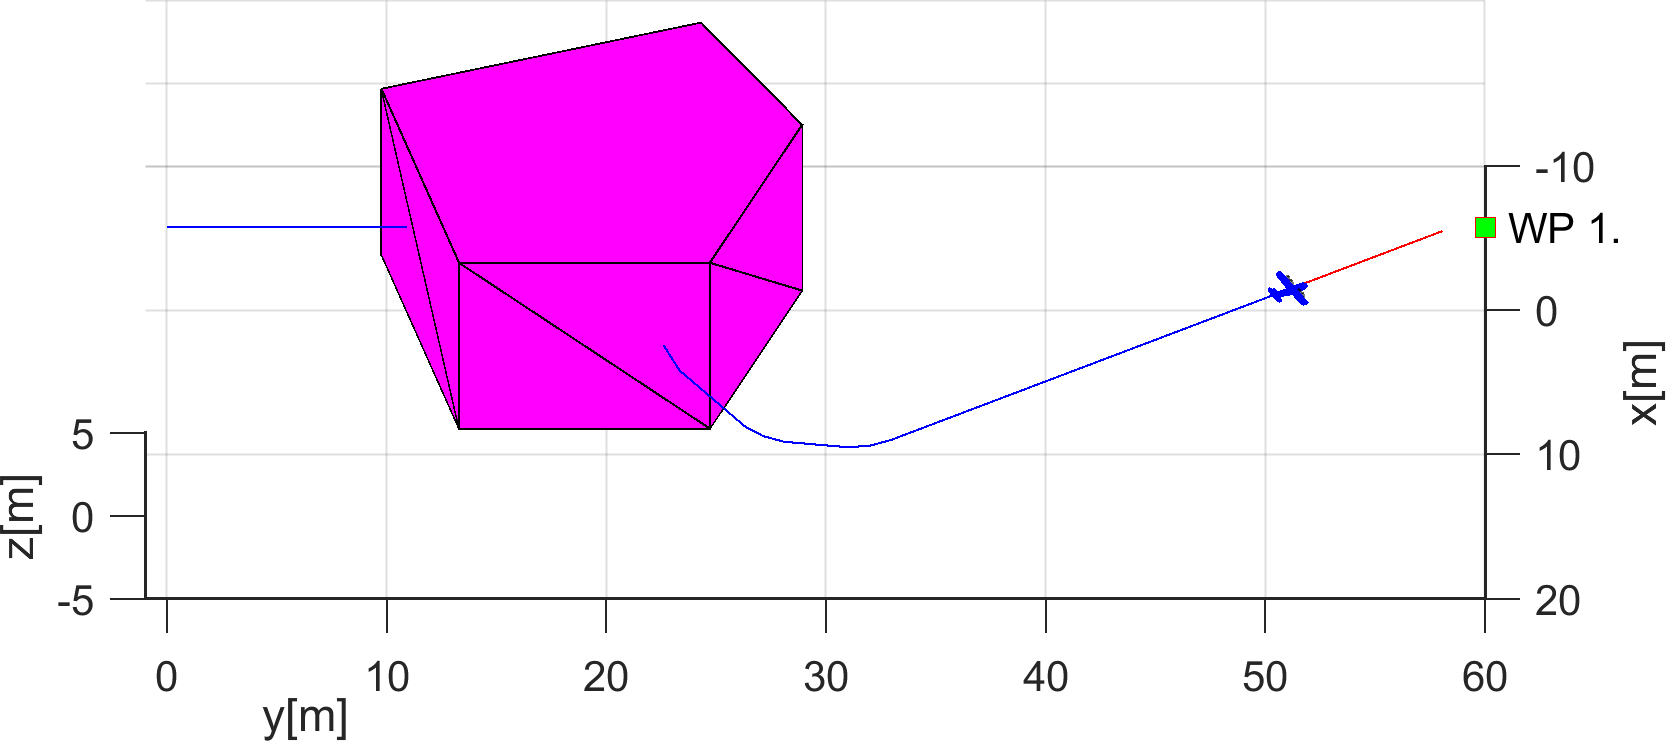
\includegraphics[width=0.9\linewidth]{\FIGDIR/NS022ConstraintsPolynomialStorm00062} 
            \caption{Waypoint reach.}
            \label{fig:stormWaypointReach}
        \end{subfigure}
        \caption{Test scenario for \emph{Storm} (Dynamic hard constraint). }
        \label{fig:testCaseStormAvoidance}
    \end{figure}
    
    \paragraph{Distance to Body/Safety Margin Evolution:} The \emph{body margin} (red line) and \emph{safety margin} (yellow line) and \emph{UAS distance to storm center} (blue line) evolution over \emph{UTM time} (x-axis) are given in (fig. \ref{fig:testCaseStormAvoidancePerformance}) The \emph{body} and \emph{safety} margin was changing according to the mutual position of the \emph{storm} and the \emph{UAS} (see tab. \ref{tab:obstacleSetStorm}). 
    
    The acceptance criteria for the \emph{hard constraint avoidance} and \emph{soft constraint avoidance} have been fulfilled. 
    
    \begin{figure}[H]
        \centering
        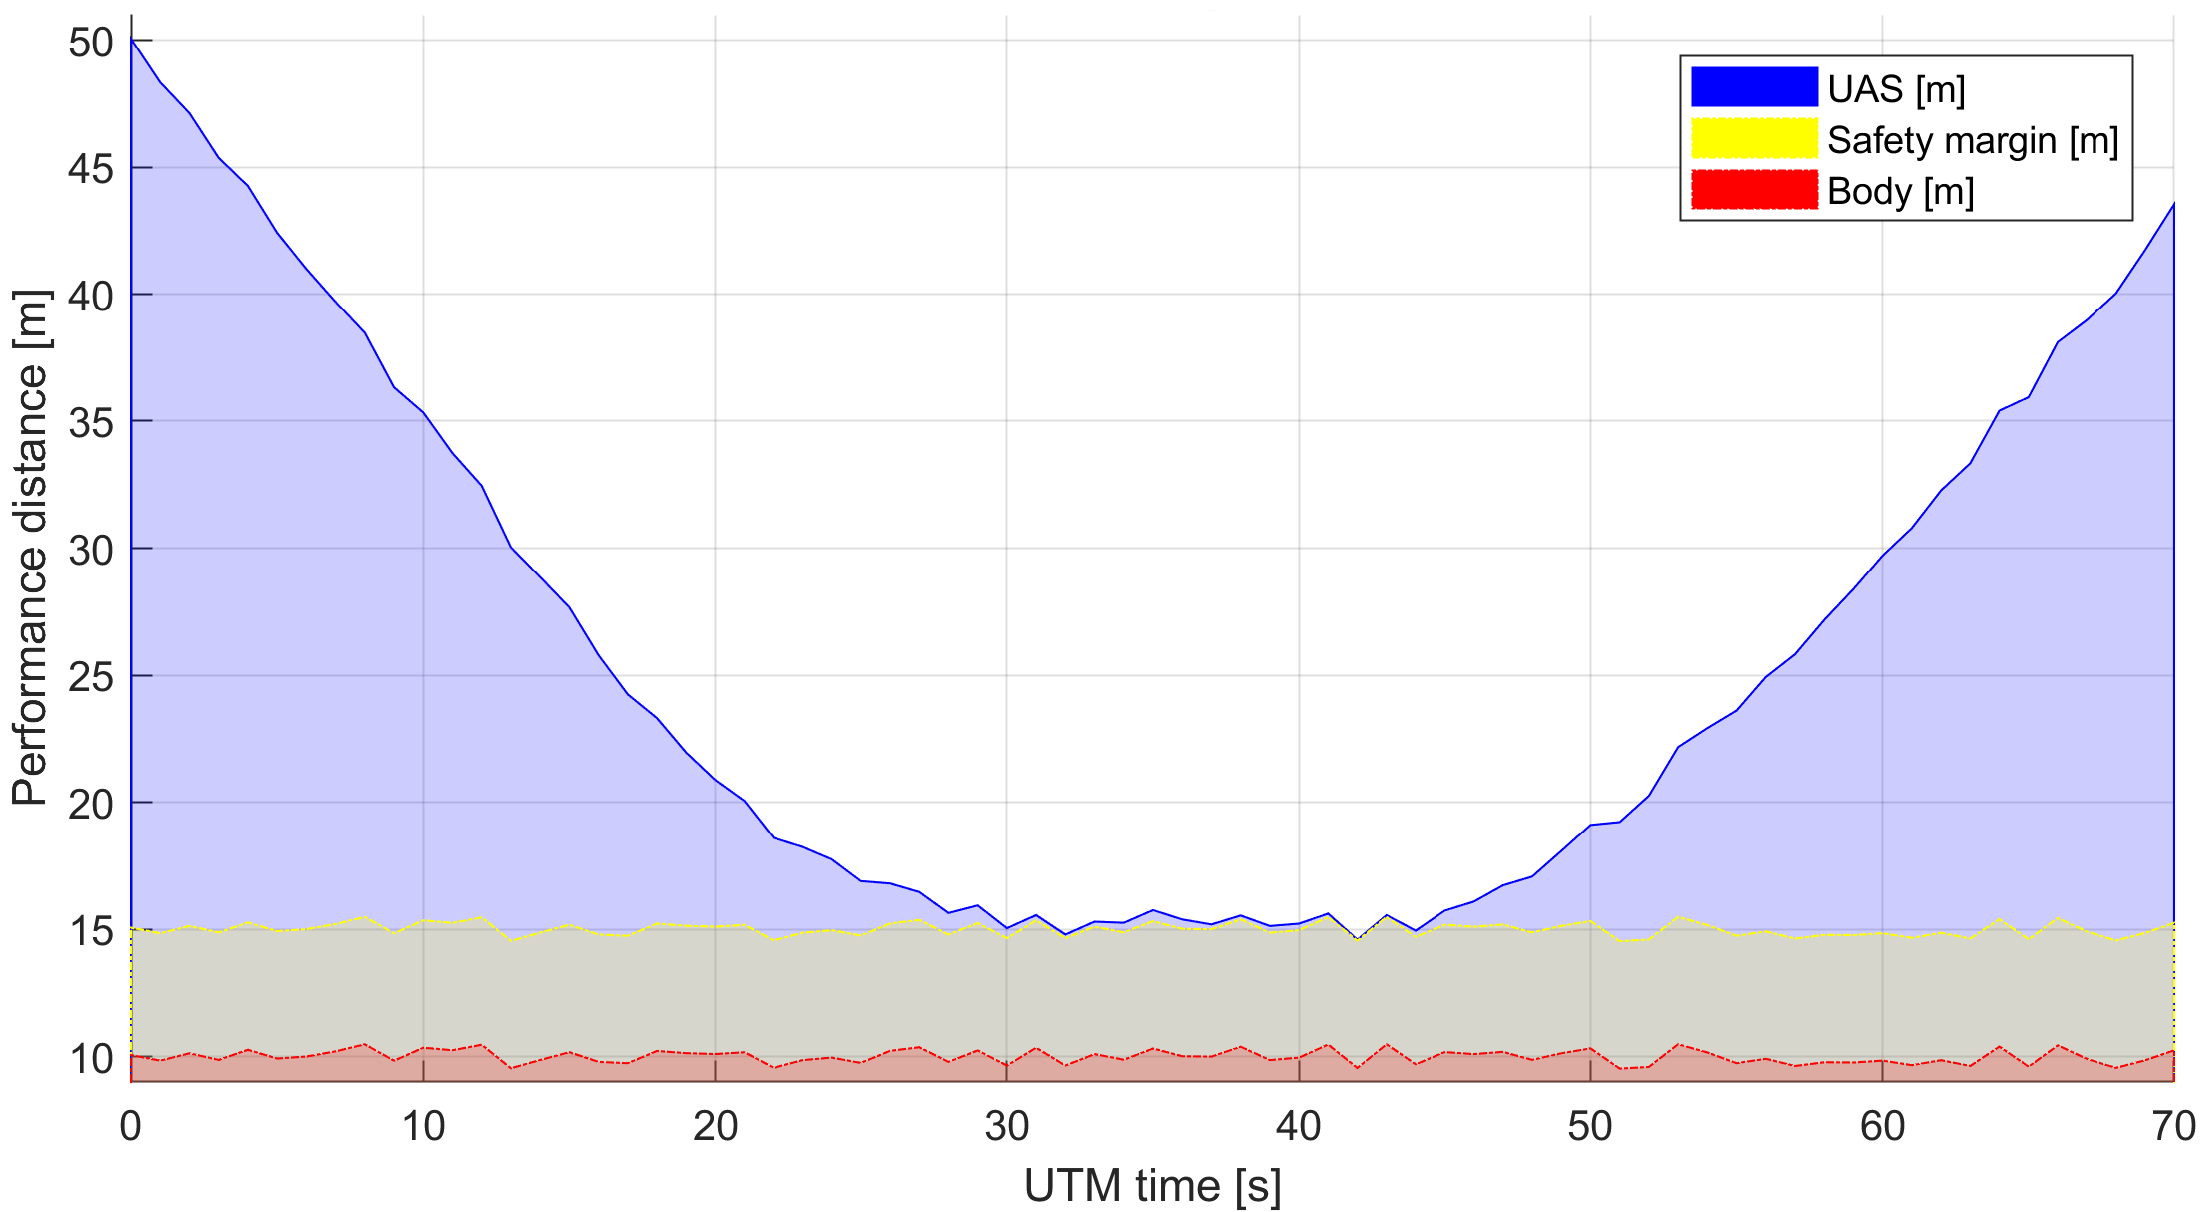
\includegraphics[width=0.8\linewidth]{\FIGDIR/NS023ConstraintsPolynomialStormPerformance} 
        \caption{Distance to body/safety margin evolution for \emph{Storm scenario}.}
        \label{fig:testCaseStormAvoidancePerformance}
    \end{figure}
    
    
    \paragraph{Distance to Body/Safety Margin Peaks:} A \emph{hard constraint} of \emph{body margin} was not breached, because the \emph{distance(UAS(t),stormBody(t))} was all time greater than \emph{0}. Thus the \emph{UAS} stayed well clear from \emph{Storm}. The summary (tab. \ref{tab:testCaseStormSafetyAndBodyMarginDistances}) shows that the \emph{minimal body margin distance} was $5.0335$ $m$, which proves \emph{avoidance of hard constraint}.
    
    A \emph{soft constraint} represented as a \emph{safety margin} (protective coating around storm body) was not breached, because the \emph{distance(UAS(t), stormBody(t)) - safetyMargin(t)} was all time greater than \emph{0}.  The summary (tab. \ref{tab:testCaseStormSafetyAndBodyMarginDistances}) show that the \emph{minimal safety margin distance} was $0.0355$ $m$, which proves \emph{avoidance of soft constraints}.
    
    \begin{table}[H]
        \centering
        \begin{tabular}{c|c||c}
        \multicolumn{2}{c||}{Parameter} & UAS 1 \\\hline\hline
        \multirow{2}{*}{Distance to Safety Margin} & min & 0.0355 \\\cline{2-3}
                                                & max & 34.9934 \\\hline
        \multirow{2}{*}{Distance to Body Margin}   & min & 5.0355 \\\cline{2-3}
                                                & max & 39.9934 
        \end{tabular}
        \caption{Distance to body/safety margin peaks for \emph{Storm scenario}.}
        \label{tab:testCaseStormSafetyAndBodyMarginDistances}
    \end{table}
    
    \paragraph{Path Tracking Performance:} The \emph{path tracking} (solid blue line) of \emph{reference trajectory} (green dashed line) between \emph{starting waypoint} (green square marked "S") and \emph{final waypoint} (green square marked "1") is portrayed in (fig. \ref{fig:testCaseStormPathTracking}). The\emph{UAS} executes \emph{horizontal right-side avoidance} of the \emph{Storm} as is preferred. 
    
    \begin{figure}[H]
        \centering
        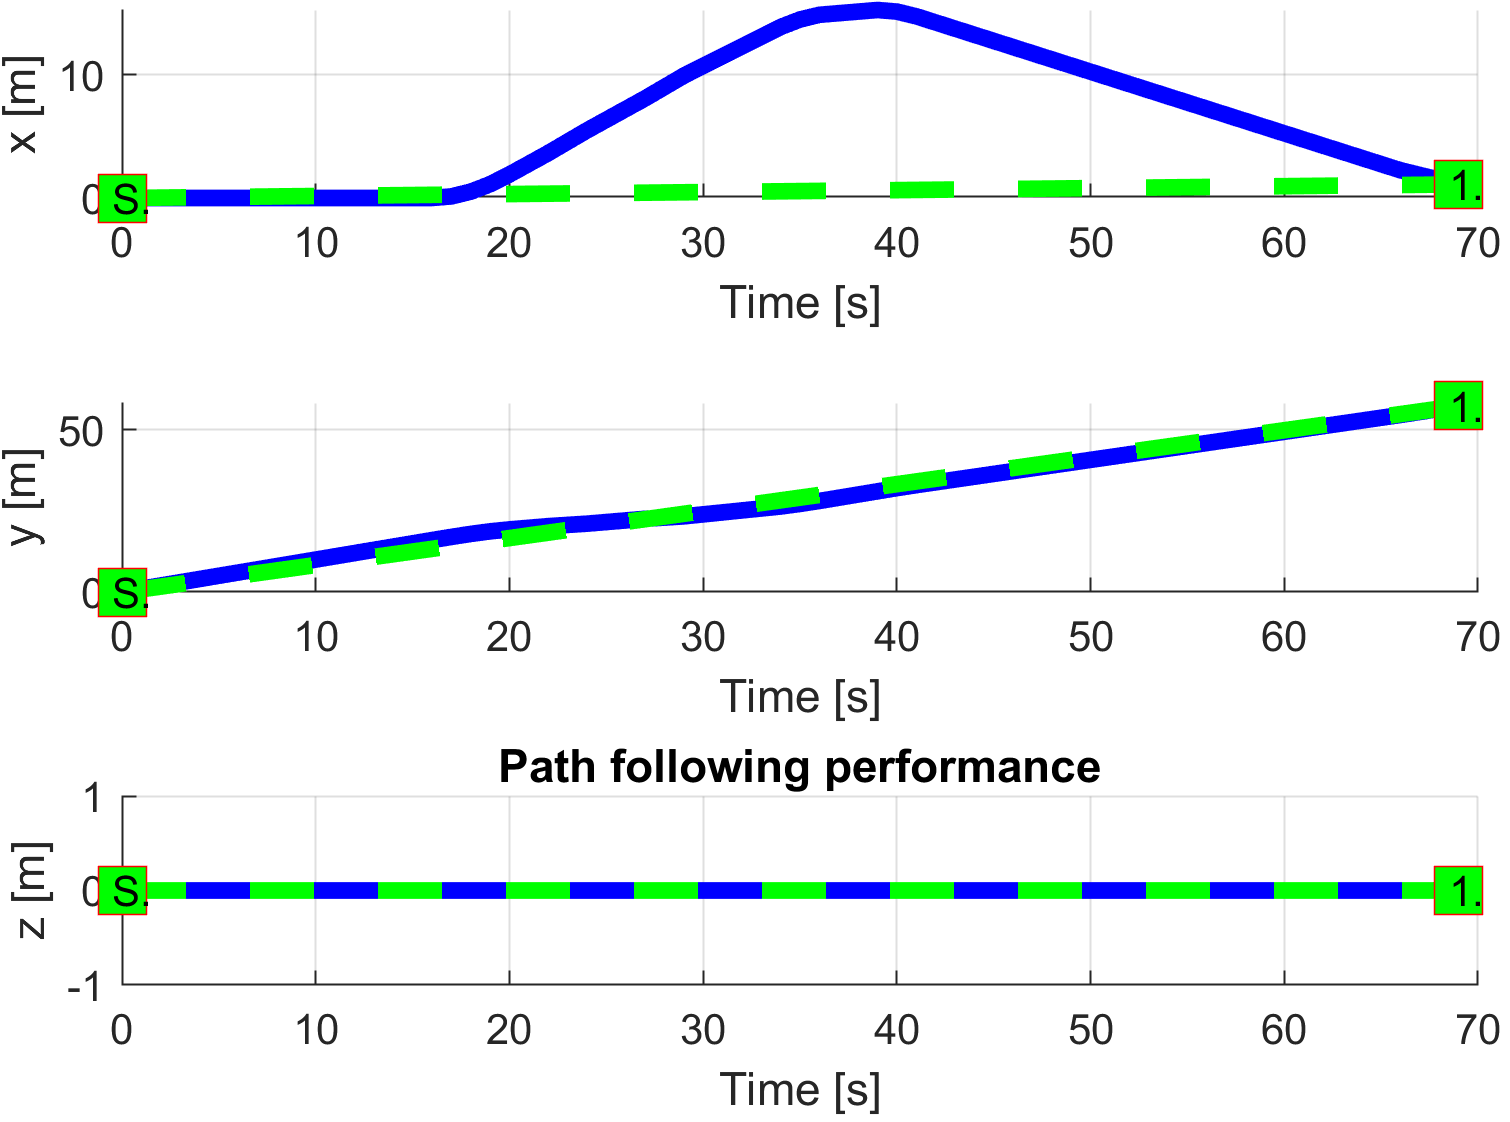
\includegraphics[width=0.55\linewidth]{\FIGDIR/NS024ConstraintsPolynomialStormPathFollowing} 
        \caption{\emph{Storm} avoidance scenario path tracking.}
        \label{fig:testCaseStormPathTracking}
    \end{figure}
    
    \paragraph{Path Tracking Deviations:} \emph{Deviations} (tab. \ref{tab:pathTrackingParametersForStormAvoidance}) are in expected ranges considering the mission plan (tab. \ref{tab:missionSetupStormScenario}) and \emph{body} and \emph{safety} margins (tab. \ref{tab:obstacleSetStorm}).
    
    \begin{table}[H]
        \centering
        \begin{tabular}{c||c}
            \multirow{2}{*}{Param.} & UAS 1\\\cline{2-2}
                            & $\mathscr{WP}_1$  \\\hline\hline
              $\max |x|$    & 15.26             \\\hline
              $\max |y|$    & 1.32             \\\hline
              $\max |z|$    & 0                 \\\hline
              $\max dist.$  & 15.76             \\
        \end{tabular}
        \caption{Path tracking properties for \emph{Storm} scenario.}
        \label{tab:pathTrackingParametersForStormAvoidance}
    \end{table}
    
    
    % 04 Storm
\paragraph{Computation Load:} The \emph{computation load} for \emph{scenario} (fig.\ref{fig:stormComputationTime}) shows used time (y-axis) over decision frame (x-axis).

The \emph{computation time} is low; it only increases slightly during  avoidance maneuver.

\begin{figure}[H]
    \centering
    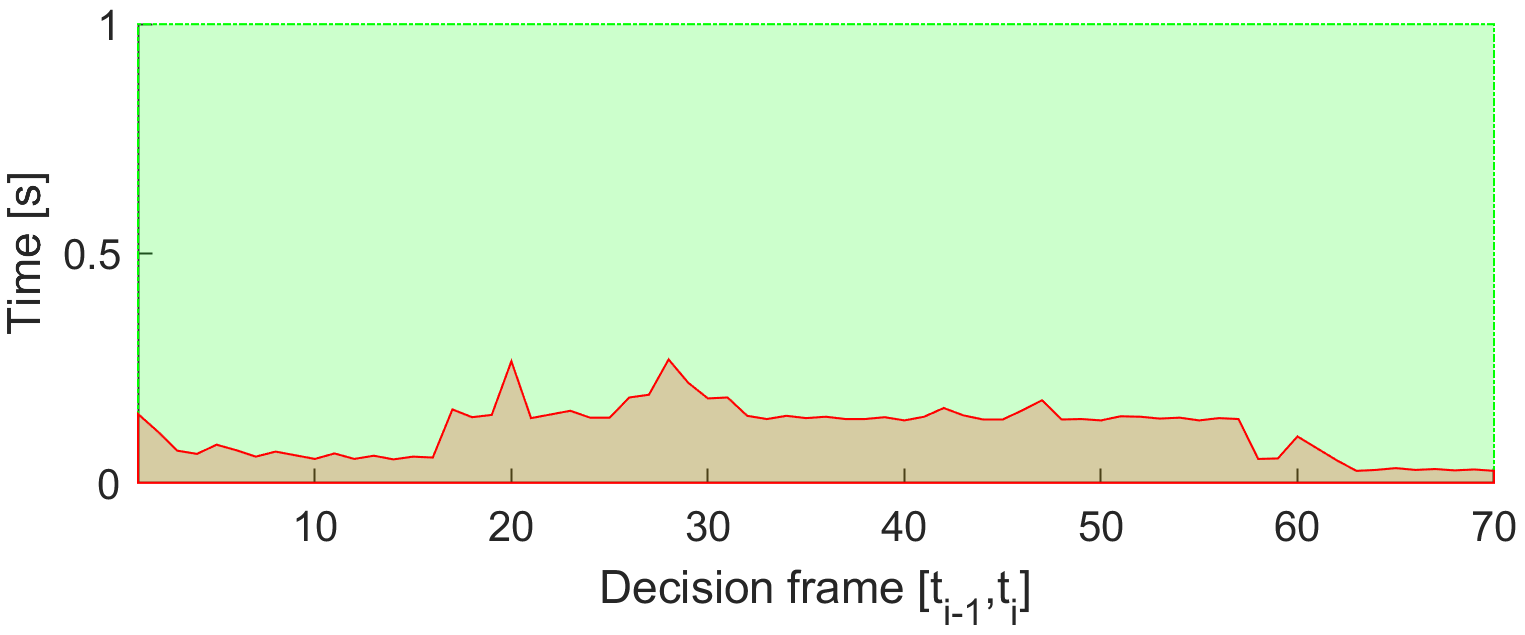
\includegraphics[width=0.65\linewidth]{\FIGDIR/NS095StormComputationTime} 
    \caption{Computation time for \emph{Maze} scenario.}
    \label{fig:stormComputationTime}
\end{figure}
    
    
